\section*{Problem 4: Solving The Augmented Solow Growth Model}
\begin{enumerate}
\item
The system of equations reads
\begin{align}
	Y(t)&=K(t)^{\alpha_K}H(t)^{\alpha_H}[A(t)L(t)]^{1-\alpha_K-\alpha_H}\\
	\dot K(t)&=s_KY(t)-\delta_kK(t)\\
	\dot H(t)&=s_HY(t)-\delta_hH(t)\\
	\dot L(t)&=nL(t)\\
	\dot A(t)&=gA(t)
\end{align}
where $\dot X(t)$ denotes the time derivative of time function $X(t)$. Now transform the system and divide all variables by $A(t)L(t)$. We denote the variables after transformation by $ x(t)=X(t)/[A(t)L(t)]$. We obtain after some steps
\begin{align}
\label{eq_y}
	 y(t)&= k(t)^{\alpha_K}h(t)^{\alpha_H}\\
\label{eq_k}
	\dot{ k}(t)&=s_K y(t)-(n+g+\delta_k) k(t)\\
\label{eq_h}
	\dot{ h}(t)&=s_H y(t)-(n+g+\delta_h) h(t)
\end{align}
At the steady-state, $\dot{ k}=\dot{ h}=0$, thus we have
\begin{align}
	s_K y(t)&=(n+g+\delta_k) k(t)\\
	s_H y(t)&=(n+g+\delta_h) h(t)
\end{align}
Substituting $ y$ into the equations and solving for $ k^*$ and $ h^*$ we obtain
\begin{align}
	 k^*&=\left(\frac{s_K}{n+g+\delta_k}\right)^{\frac{1-\alpha_H}{1-\alpha_K-\alpha_H}}
				\left(\frac{s_H}{n+g+\delta_h}\right)^{\frac{\alpha_H}{1-\alpha_K-\alpha_H}}\\
	 h^*&=\left(\frac{s_H}{n+g+\delta_h}\right)^{\frac{1-\alpha_K}{1-\alpha_K-\alpha_H}}
				\left(\frac{s_K}{n+g+\delta_k}\right)^{\frac{\alpha_K}{1-\alpha_K-\alpha_H}}
\end{align}
Now substituting in our parameterization, we obtain
\begin{equation}
	k^*\approx5.7932,\qquad
	h^*\approx8.5194.
\end{equation}

\item
Substituting Eq.\eqref{eq_y} into Eq.\eqref{eq_k} and \eqref{eq_h}, and letting $\dot k=\dot h=0$, we obtain at steady state
\begin{align}
	f_1(k,h):=s_K k(t)^{\alpha_K}h(t)^{\alpha_H}-(n+g+\delta_k) k(t)&=0\\
	f_2(k,h):=s_H k(t)^{\alpha_K}h(t)^{\alpha_H}-(n+g+\delta_h) h(t)&=0
\end{align}
Dropping all time arguments, the Jacobian is given by
\begin{align}
	\mathcal J&=
		\begin{pmatrix}
			\frac{\partial f_1}{\partial k} & \frac{\partial f_1}{\partial h}\\
			\frac{\partial f_2}{\partial k} & \frac{\partial f_2}{\partial h}
		\end{pmatrix}\\
	&=
		\begin{pmatrix}
			\alpha_Ks_Kk^{\alpha_K-1}h^{\alpha_H}-(n+g+\delta_k) & \alpha_Hs_Kk^\alpha_Kh^{\alpha_H-1}\\
			\alpha_Ks_Hk^{\alpha_K-1}h^{\alpha_H} & \alpha_Hs_Hk^\alpha_Kh^{\alpha_H-1}-(n+g+\delta_k)
		\end{pmatrix}
\end{align}

\item
For $\epsilon=\delta=0.001$, convergence is reported after 5 iterations, with infinite norm difference from the true value being 3.133e-11.\\
For $\epsilon=\delta=1e-20$, convergence is reported after 7 iterations, with infinite norm difference from the true value being 7.105e-15.

\item
For $\epsilon=\delta=0.001$, convergence is reported after 21 iterations, with infinite norm difference from the true value being 0.00019.\\
For $\epsilon=\delta=1e-20$, convergence is reported after 29 iterations, with infinite norm difference from the true value being 1.776e-15.

\item
For $\epsilon=\delta=0.001$, convergence is reported after 21 iterations, with infinite norm difference from the true value being 0.00019.\\
For $\epsilon=\delta=1e-20$, convergence is reported after 29 iterations, with infinite norm difference from the true value being 1.776e-15.

\item
Convergence of $k$ and $h$ are shown in the figure below. Agents start to accumulate both types of capital since the beginning, at a decreasing rate when approaching the steady state. They stop capital accumulation after reaching the steady state and continue to produce with the same amount of captial.\\
\begin{figure}[htbp]
\begin{center}
	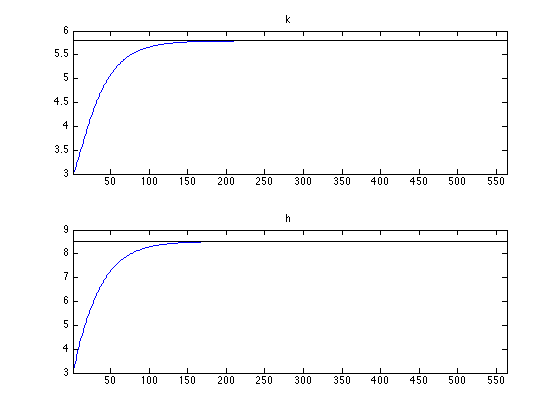
\includegraphics[width=10cm]{Figure/Q4_6.png}	
\caption{Convergence of $k$ and $h$}
\end{center}
\end{figure}
\end{enumerate}